\documentclass[a4paper, USenglish]{llncs}

\bibliographystyle{plainurl}

\usepackage{todonotes}
\usepackage{graphicx}
\usepackage[basic]{complexity}
\usepackage{wrapfig}
\usepackage{subfig}
\usepackage{xspace}
\usepackage{hyperref}
\usepackage{amsmath, amssymb}

\title{Maximizing Ink in Symmetric Partial Edge Drawings of $k$-plane Graphs}
\author{Fabian Klute \and Soeren Nickel \and Martin~N\"ollenburg}
\institute{Algorithms and Complexity Group, TU Wien, Vienna, Austria \email{[fklute|noellenburg]@ac.tuwien.ac.at, soeren.nickel@tuwien.ac.at}}

\newcommand{\martin}[1]{\todo[inline,color=blue!40]{MN: #1}}
\newcommand{\fabian}[1]{\todo[inline,color=pink!40]{FK: #1}}
\newcommand{\birgit}[1]{\todo[inline,color=red!40]{BS: #1}}
\newcommand{\michael}[1]{\todo[inline,color=green!40]{MH: #1}}
\newcommand{\soeren}[1]{\todo[inline,color=orange!40]{SN: #1}}

\newcommand{\ped}{\ensuremath{\textsc{PED}}\xspace}
\newcommand{\maxsped}{\ensuremath{\textsc{MaxSPED}}\xspace}
\newcommand{\ppsat}{\ensuremath{\textsc{Planar 3-Sat}}\xspace}
\newcommand{\sollong}{\ensuremath{\textit{long}}\xspace}
\newcommand{\solmid}{\ensuremath{\textit{mid}}\xspace}
\newcommand{\solshort}{\ensuremath{\textit{short}}\xspace}

\begin{document}
	\maketitle
	
	\begin{abstract}
		Partial edge drawing (PED) is a drawing style for non-planar graphs, in which edges are drawn only partially as pairs of opposing stubs on the respective end-vertices. 
		In a PED, by erasing the central parts of edges, all edge crossings and the resulting visual clutter are hidden in the undrawn parts of the edges.
		We study symmetric partial edge drawings (SPEDs), in which the two stubs of each edge are required to have the same length. 
		It is known that maximizing the ink (or the total stub length) when transforming a straight-line drawing with crossings into a SPED is tractable for 2-plane input drawings, but generally \NP-hard.
		We show that the problem remains \NP-hard even for 3-plane input drawings.
		Yet, for $k$-plane input drawings whose edge intersection graph forms a collection of trees or cacti we present efficient algorithms for ink maximization.
	\end{abstract}

	\section{Introduction}
	
	Visualizing non-planar graphs as node-link diagrams is challenging due to the visual clutter caused by edge crossings. The layout readability deteriorates as the edge density and thus the number of crossings increases.
	Therefore alternative layout styles are necessary for non-planar graphs.
	A radical approach first used in applied network visualization work by Becker et al.~\cite{bew-vnd-95} is to start with a traditional straight-line graph drawing and simply drop a large central part of each edge and with it many of the edge crossings.
	This idea relies on the closure and continuation principles in Gestalt theory, which imply that humans can still see a full line segment based only on the remaining edge stubs by filling in the missing information in our brains.
	User studies have confirmed that such drawings remain readable while reducing clutter significantly~\cite{bvkw-epdldge-12,bkl-us-15}.
	
	\begin{figure}
		\centering
		\subfloat{
			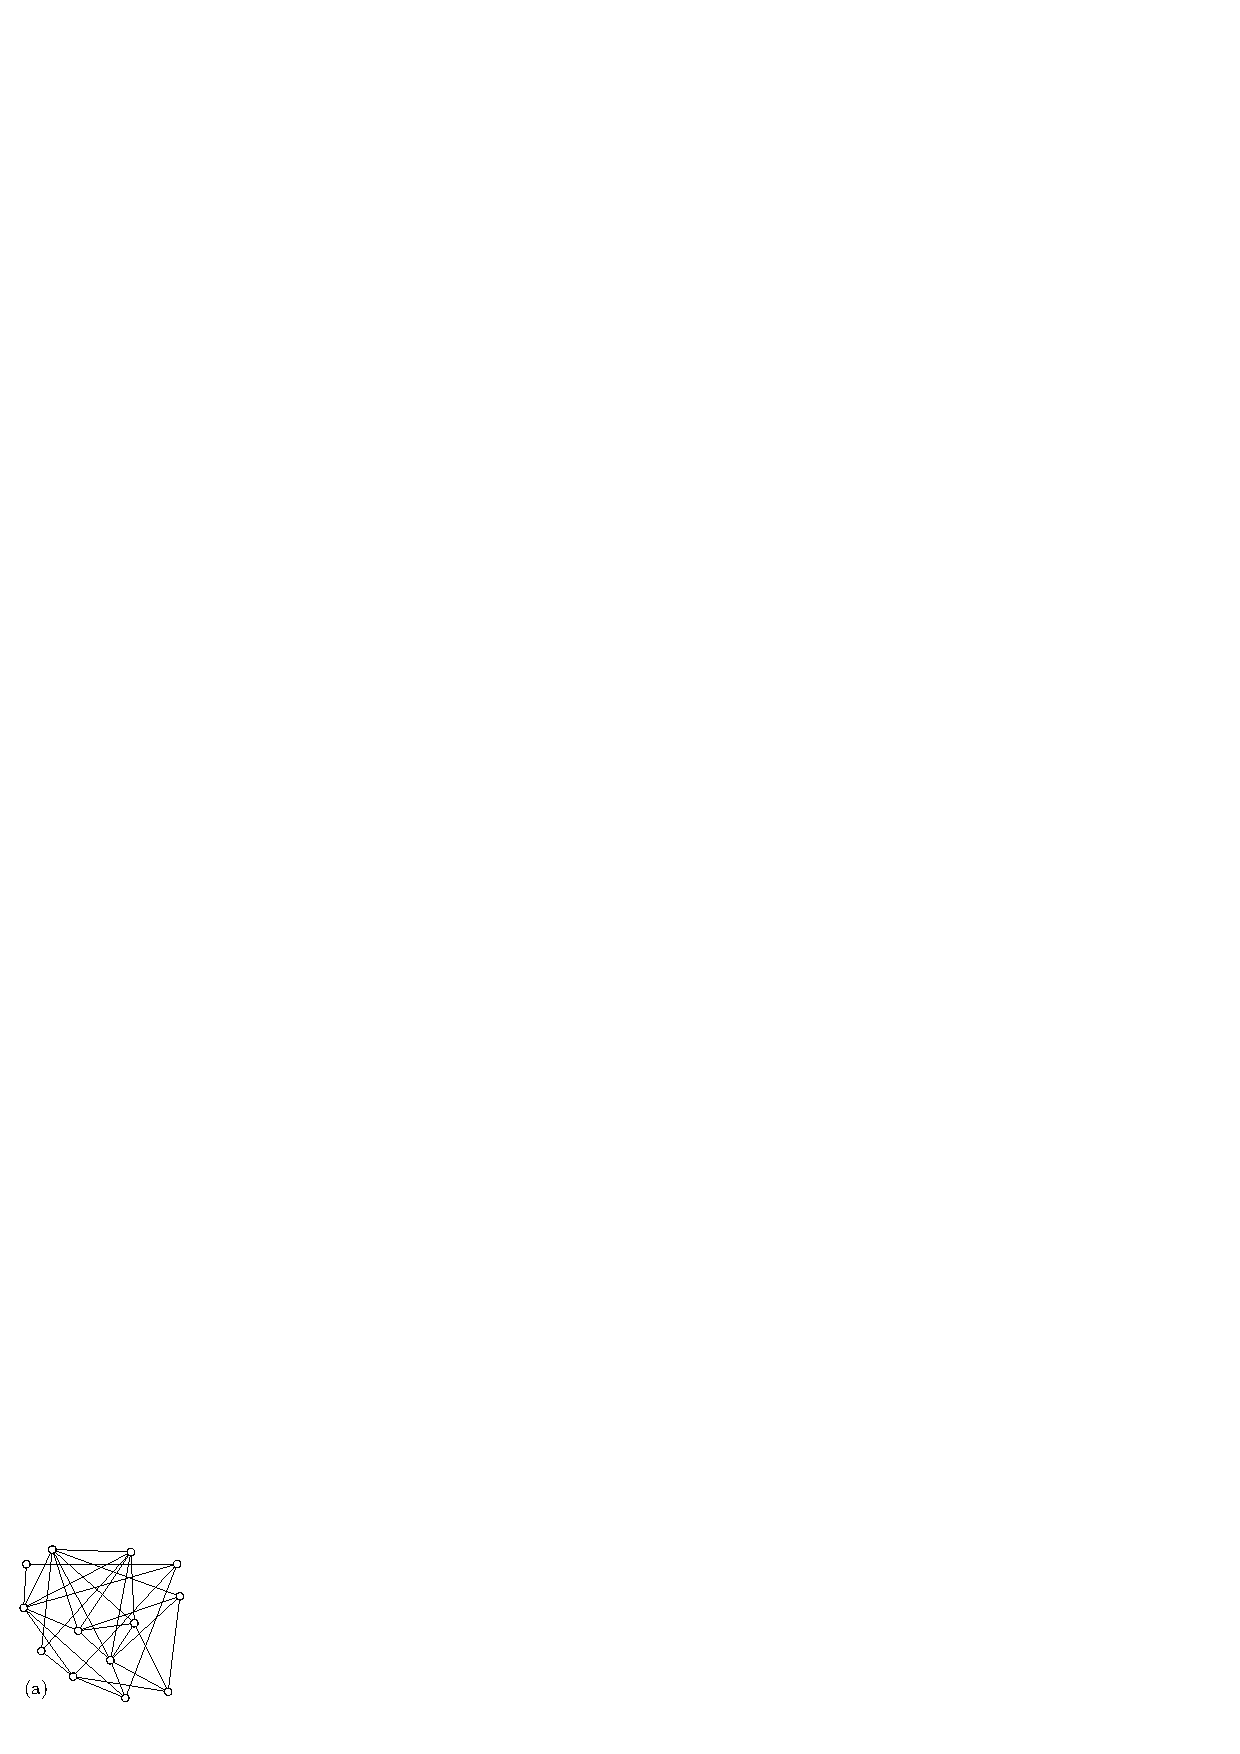
\includegraphics{figures/export_full}
		}
		\subfloat {
			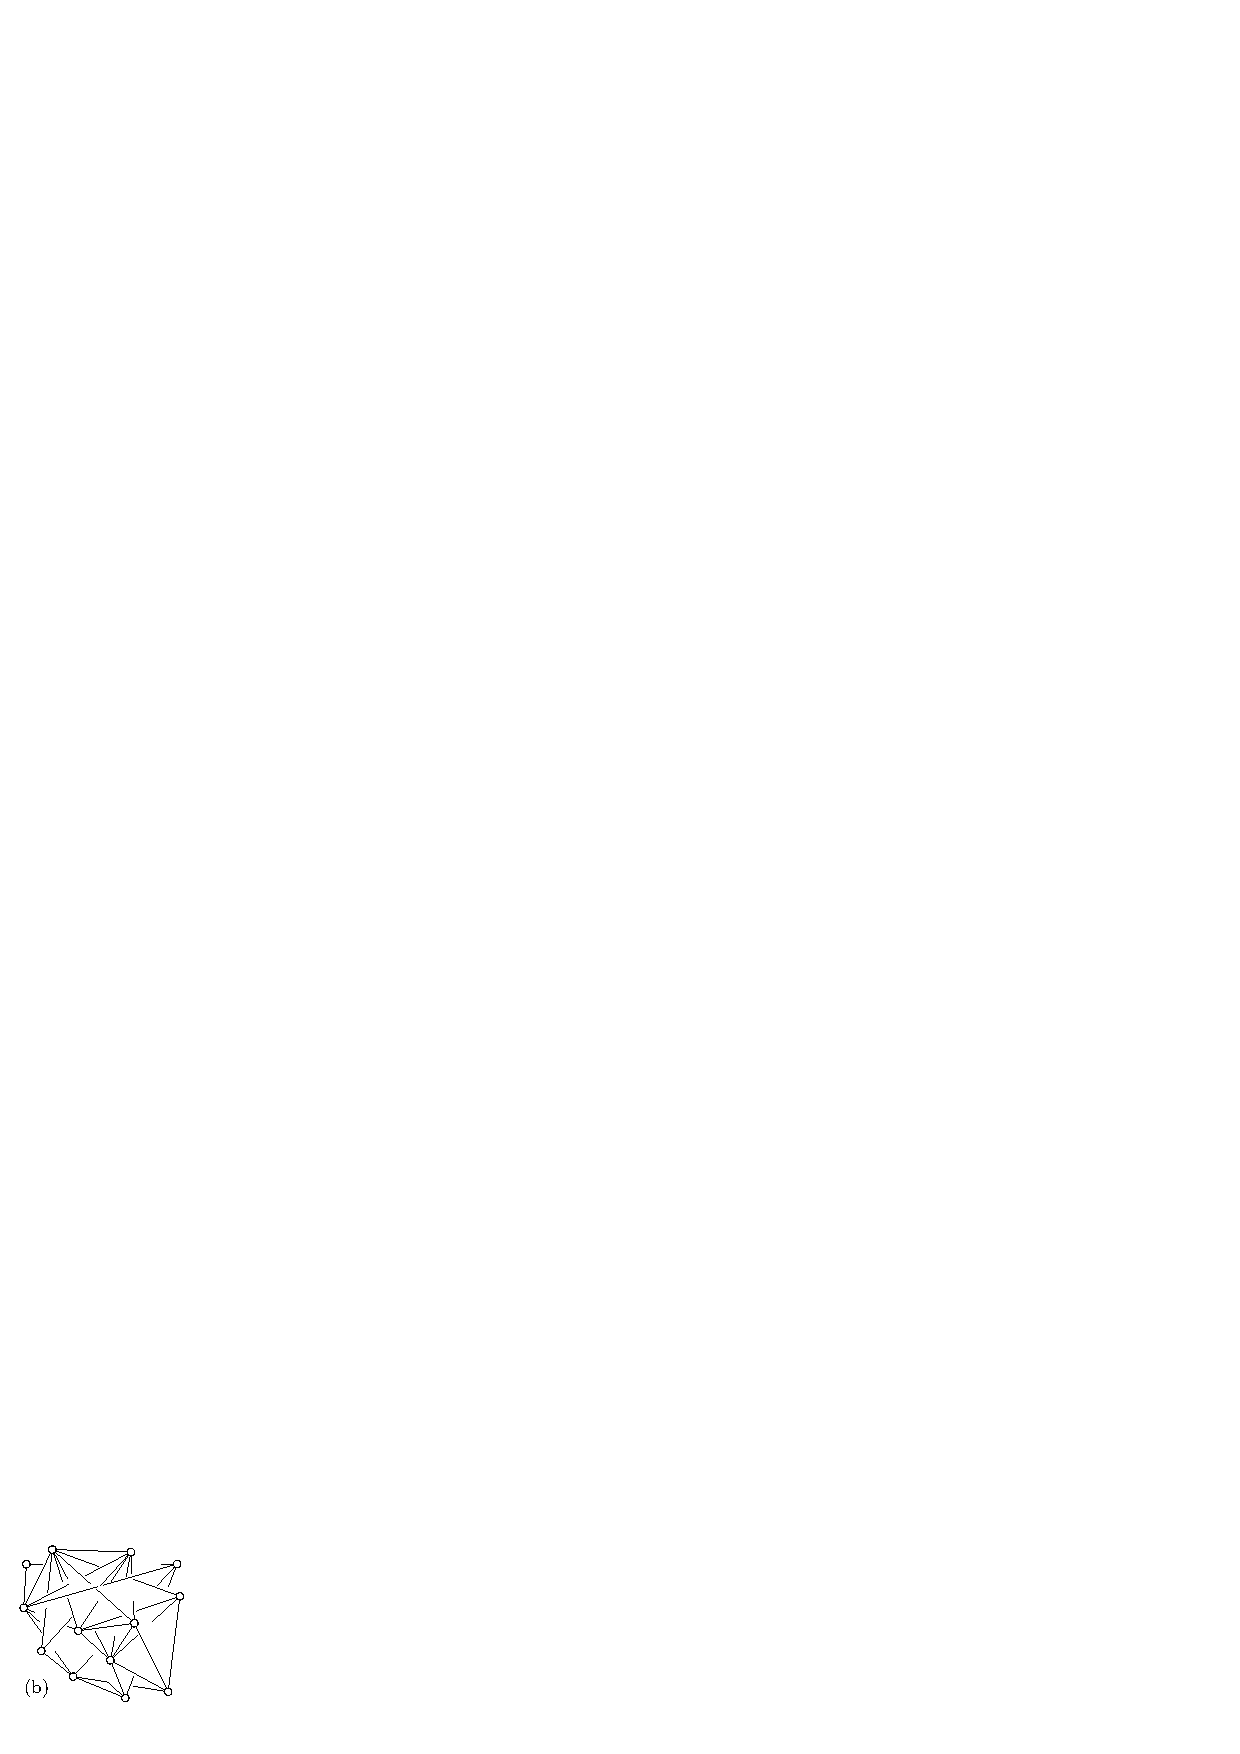
\includegraphics{figures/export_alpha_nontouching}
		}	
		\caption{A straight-line graph drawing (a) and a maximum-ink symmetric partial edge drawing (b) of the same graph.}
		\label{fig:examples}
	\end{figure}
	
	
	The idea of drawing edges only partially has been formalized in graph drawing as follows~\cite{bk-ecbe-12}. 
	A \emph{partial edge drawing (PED)} is a graph drawing that maps vertices to points and edges to pairs of crossing-free edge stubs of positive length pointing towards each other.
	These edge stubs are obtained by erasing one contiguous central piece of the straight-line segment connecting the two endpoints of each edge.
	In other words each straight-line edge is divided into three parts, of which only the two outer ones are drawn (see Fig.~\ref{fig:examples}).
	More restricted and better readable~\cite{blmt-pedhmitc-16} variations of PEDs are \emph{symmetric} PEDs, in which both stubs of an edge must have the same length (see Fig.~\ref{fig:examples}(b)), and \emph{homogeneous} PEDs, in which the ratio of the stub length to the total edge length is the same for all edges.
	The natural optimization problem in this formal setting is \emph{ink maximization}, i.e., maximizing the total stub length, so that as much information as possible is given in the drawing while all crossings disappear in the negative background space. 	
	
	We study the ink maximization problem for symmetric partial edge drawings (SPEDs) with a given geometric input drawing.
	This problem is known as \maxsped. 
	Bruckdorfer and Kaufmann~\cite{bk-ecbe-12} presented an integer linear program for solving \maxsped. 
	Later, Bruckdorfer et al.~\cite{bcgkmn-pped-17} gave an $O(n \log n)$-time algorithm for \maxsped on the class of 2-plane input drawings (no edge has more than two crossings), where $n$ is the number of vertices, and an efficient 2-approximation algorithm for the dual problem of minimizing the amount of erased ink for arbitrary input drawings.
	Bruckdorfer~\cite{b-sgh-15} further gives an \NP-hardness proof for \maxsped.
	
	\medskip
	
	\noindent\textbf{Contribution.} We extend the results of Bruckdorfer et al.~\cite{bcgkmn-pped-17} on 2-plane geometric graph drawings to $k$-plane graph drawings for $k > 2$. 
	In particular, we show that \maxsped is \NP-hard even for 3-plane input drawings. 
	However, for $k$-plane graph drawings whose edge intersection graphs are collections of trees or cacti (which have maximum degree $k$), we give polynomial-time algorithms for solving \maxsped.
	
	\section{Preliminaries}\label{sec:preliminaries}
	
	Throughout the paper let $ G $ be a \emph{simple graph} with edge set $ S = \{s_1,\dots,s_m\}$ and $ \Gamma $ a straight line drawing of $ G $ in the plane. We call $ \Gamma $ \emph{$ k $-plane} if every edge $ s_i \in S $ is crossed by at most $ k $ other edges from $ S $ in $ \Gamma $. We use the terms edge in $ S $ and segment in $ \Gamma $ interchangeably. %, since our input is always a graph $G$ with a given drawing $ \Gamma $. 
	Hence we can also interpret $S$ as a set of line segments.
	
	The \emph{intersection graph} $ C = (V,E) $ of $ \Gamma $ is the graph containing a vertex $v_i$ in $ V $ for every $ s_i \in S $ and an edge $ v_i v_j \in E $ between vertices $ v_i, v_j \in V $ if the corresponding edges $ s_i, s_j \in S $ intersect in $ \Gamma $. 
	We also denote the segment in $S$ corresponding to a vertex $v \in V$ by $s(v)$.
	Observe that the intersection graph $ C $ of a $ k $-plane drawing $ \Gamma $ has maximum degree~$ k $.  
	%
	Using a standard sweep-line algorithm, computing the intersection graph $C$ of a set of $m$ line segments takes $O(m \log m + |E|)$ time~\cite{bcko-cgaa-08}, where $|E|$ is  the number of intersections.
	
	A \emph{symmetric partial edge drawing} (SPED) $D$ of $\Gamma$ draws a fraction $0 < f_s \le 1$ of each edge $s = uv \in S$ by drawing two symmetric edge stubs at $u$ and $v$ of length $f_s \cdot |s|/2$ each. 
	No two stubs in $D$ may intersect.
	The \emph{ink} or \emph{ink value}  $I(D)$ of a SPED $D$ is the total stub length $I(D) = \sum_{s \in S} f_s |s|$.
	In the problem \maxsped, the task is to find for a given drawing~$\Gamma$ a SPED $D^*$ such that its ink $I(D^*)$ is maximum over all SPEDs.
	
	\section{Hardness of \maxsped for $k\ge3$}\label{sec:hardness}
	
	In this section we close the gap between the known hardness of \maxsped~\cite{b-sgh-15} and the polynomial-time algorithm for 2-plane drawings~\cite{bcgkmn-pped-17} as stated in the following theorem.
	
	\begin{theorem}\label{thm:hard}
		\maxsped is \NP-hard even for 3-plane graph drawings.
	\end{theorem}
	\begin{proof}
		We reduce from the \NP-hard problem \ppsat~\cite{l-pftu-82} using similar ideas as in Bruckdorfer's general proof of the hardness of \maxsped~\cite{b-sgh-15}. 
		Let $\phi$ be a planar 3-Sat formula with $n$ variables $\{x_1, \dots, x_n\}$ and $m$ clauses $\{c_1, \dots, c_m\}$, each consisting of three literals.
		We can assume that $\phi$ comes with a planar drawing of its variable-clause graph $H_\phi$, which has a vertex for each variable $x_i$ and a vertex for each clause $c_j$.
		Each clause vertex is connected to the three variables appearing in the clause.
		In the drawing of $H_\phi$ all variable vertices are placed on a horizontal line and the clause vertices connect to the adjacent variable vertices either from above or from below the horizontal line.
		In our gadget-based reduction we mimic the drawing of $H_\phi$ by creating a 3-plane drawing $\Gamma_\phi$ as a set of line segments of uniform length and a value $L$ such that $\Gamma_\phi$ has a SPED with ink at least $L$ if and only if $\phi$ is satisfiable.
		Figure~\ref{fig:gadget_connection} shows a sketch of the gadgets.
		\begin{figure}
			\centering
			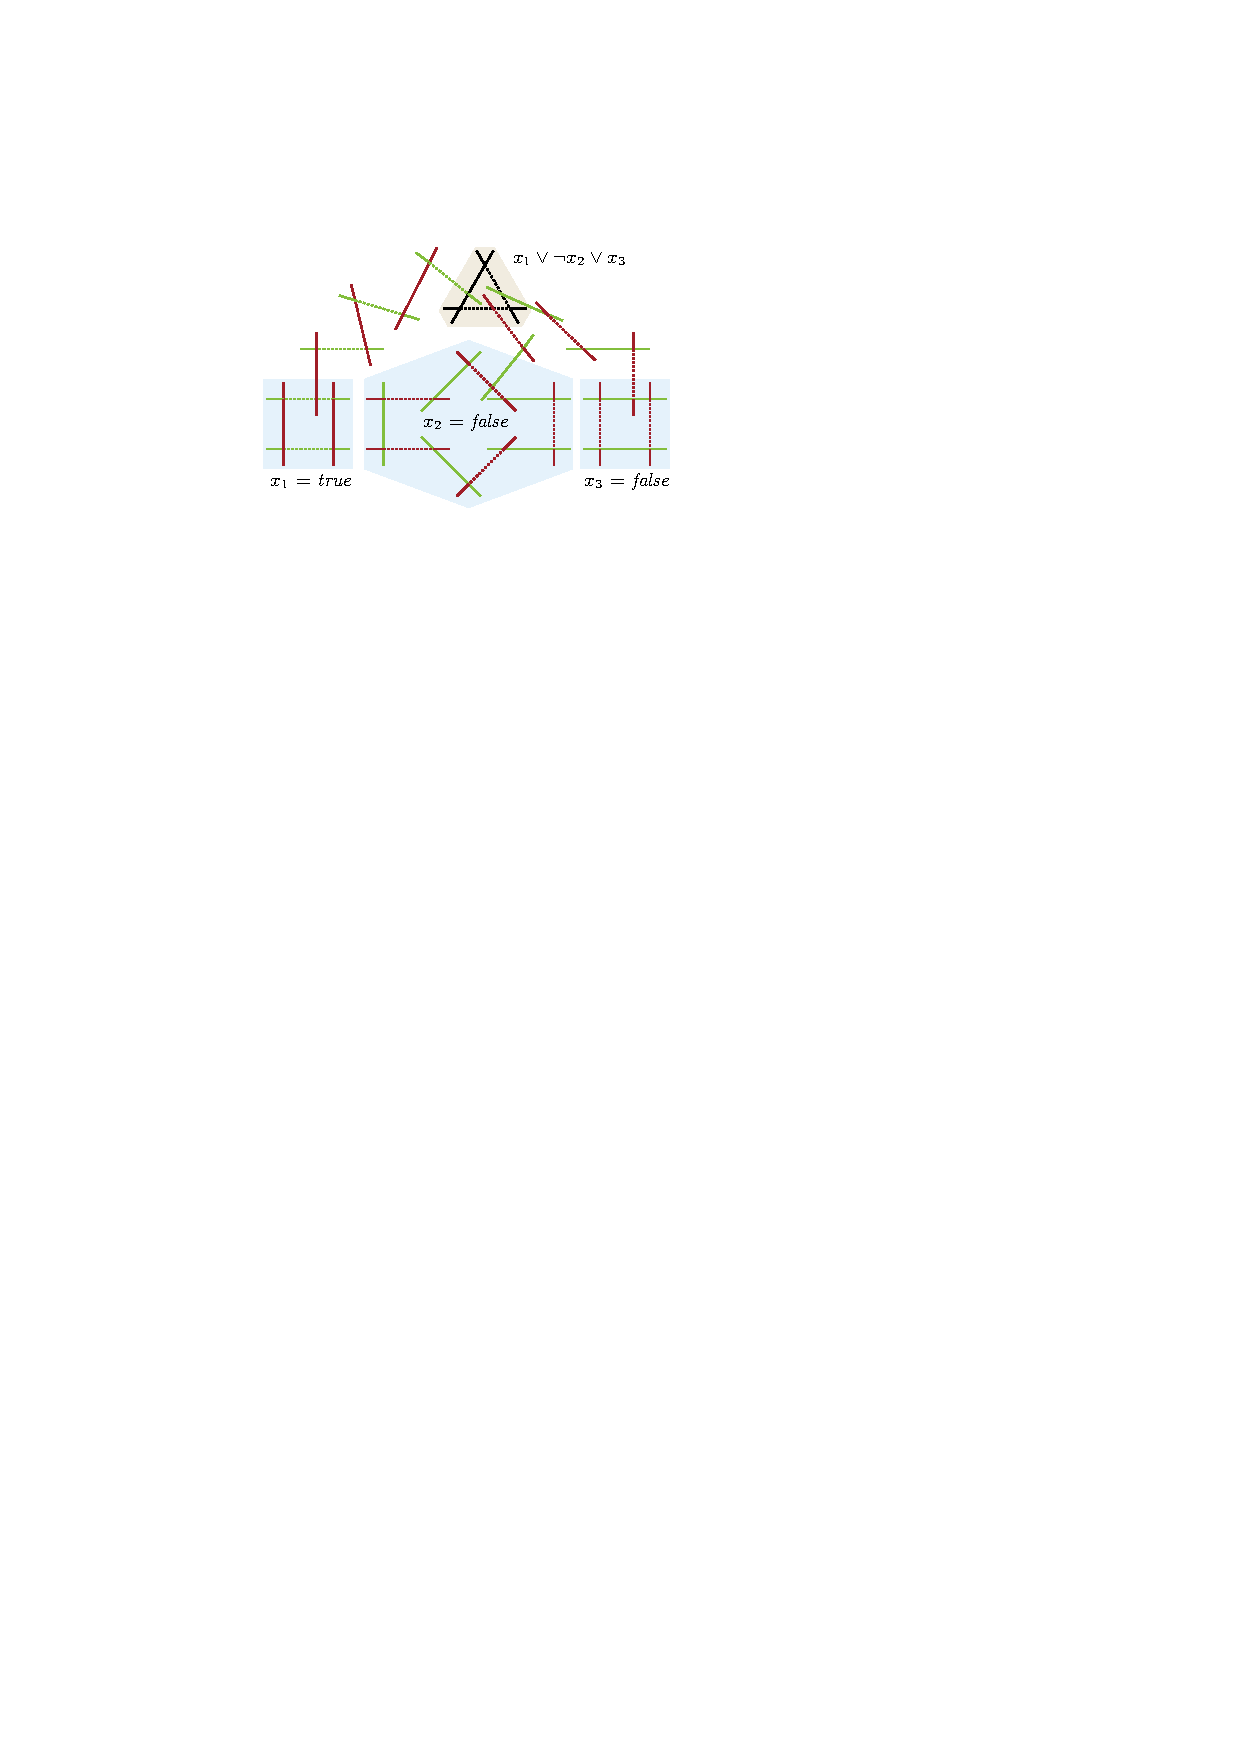
\includegraphics{figures/Reduction_visual}
			\caption{Example of three variable gadgets and a satisfied clause gadget. Dotted parts do not belong to the SPED.}
			\label{fig:gadget_connection}
		\end{figure}
		All segments in the gadgets are of length 5.
		We use pairs of intersecting segments, alternatingly colored red and green.
		The intersection point of each red-green segment pair is at distance 1 from an endpoint.
		Thus, the maximum amount of ink contributed by such a pair is 7 (one full segment of length 5 and the other one with two stubs of length 1 each).
		
		Each variable gadget is a cycle of segment pairs, with at least one pair for each occurrence of the variable in $\phi$, see Fig.~\ref{fig:gadget_connection}. 
		Observe that this cycle has exactly two ink-maximal SPEDs: either all red edges are full segments and all green edges are length-1 stubs or vice versa.
		We associate the configuration with green stubs and full red segments with the value \emph{true} and the configuration with full green segments and red stubs with the value \emph{false}.
		
		For each clause we construct a triple of mutually intersecting segments, see the gadget on yellow background in the upper part of Fig.~\ref{fig:gadget_connection}.
		Again, their intersection points are at distance~1 from the endpoints.
		It is clear that in such a clause triangle at most one of the three segments can be fully drawn, while the stubs of the other two can have length at most~1.
		Hence, the maximum amount of ink in a SPED contributed by a clause gadget is~9.
		
		Finally, we connect variable and clause gadgets in such a way that a clause gadget can contribute its maximum ink value of 9 if and only if the clause is satisfied by the selected truth assignment to the variables.
		For a positive (negative) literal, we create a path of even length between a green (red) edge of the variable gadget and one of the three edges of the clause gadget as shown in Fig.~\ref{fig:gadget_connection}.
		The first edge $s$ of this path intersects the corresponding variable edge $s'$ such that $s'$ is split into a piece of length 2 and a piece of length 3, whereas $s$ is split into a piece of length 1 and a piece of length 4.
		The last edge of the path intersects the corresponding clause edge with the same length ratios.
		The path itself consists of a chain of red-green segment pairs, so each pair contributes an ink value of at most~7.
		
		Since the drawing of $H_\phi$ has polynomial size, the number of segments created in the reduction is polynomial. 
		Further, no segment intersects more than three other segments, so the constructed drawing is 3-plane. 
		
		For the correctness of the reduction, let $L$ be the ink value obtained by counting 7 for each red-green segment pair and 9 for each clause gadget. 
		First assume that $\phi$ has a satisfying truth assignment and put each variable gadget in its corresponding state.
		For each clause, select exactly one literal with value \emph{true} in the satisfying truth assignment. 
		We draw the clause segment that connects to the selected literal as a full segment and the other two as length-1 stubs.
		Recall that the literal paths are oriented from the variable gadget to the clause gadget.
		Since the last segment of the selected literal path must be drawn as length-1 stubs, the only way of having a maximum contribution of that path is by alternating stubs and full segments.
		Hence, the first segment of the path must be a full segment.
		But because the variable is in the state that sets the literal to \emph{true}, the intersecting variable segment is drawn as two stubs and the path configuration is valid.
		For the two non-selected literals, we can draw the last segments of their paths as full segments, as well as every segment at an even position, while the segments at odd positions are drawn as stubs. 
		This is compatible with any of the two variable configurations and proves that we can indeed achieve ink value~$L$.
		
		Conversely, assume that we have a SPED with ink value $L$. 
		By construction, every red-green segment pair and every clause gadget must contribute its respective maximum ink value.
		In particular, each variable gadget is either in state \emph{true} or \emph{false}.
		We claim that this truth assignment satisfies $\phi$.
		For each clause, one segment must have full length and as argued before the path connecting that segment to a variable gadget must have all segments at even positions as length-1 stubs and all segments at odd positions as full segments. 
		In particular, the first segment of the literal path is fully drawn and therefore, in a SPED with ink $L$, the intersecting segment of the variable cannot be fully drawn.
		In fact, it must be drawn as length-1 stubs for otherwise the variable gadget would not contribute its maximum ink value.
		But then by construction, the selected variable value sets our literal to \emph{true}.	
	\end{proof}
	
	\section{Two polynomial special cases}
	
	Section~\ref{sec:hardness} showed that \maxsped is generally \NP-hard for $k \ge 3$. 
	Now we consider the special case that the intersection graph of the $k$-plane input drawing is a tree or a cactus. In both cases we present polynomial-time dynamic programming algorithms. Let $ C = (V,E) $ be the intersection graph of a given drawing $\Gamma$ of graph $ G $ as defined in Section~\ref{sec:preliminaries}. 
	Let $ u \in V $ and $ \delta  = \deg(u) $. 
	Then for the corresponding segment $ s(u) \in S $ there are $ \delta + 1 $ relevant stub pairs including the whole segment, see Fig.~\ref{fig:tree}. 
	Let $ \ell_1(u), \dots, \ell_\delta(u) \in \mathbb{R}_+$ be the stub lengths induced by the intersection points of $s(u)$ with the segments of the neighbors of $u$,  sorted from shorter to longer stubs. We define  $ \ell_0(u) $ as the length of the whole segment $ s(u) $. 
	
	\begin{figure}[tbp]
		\centering
		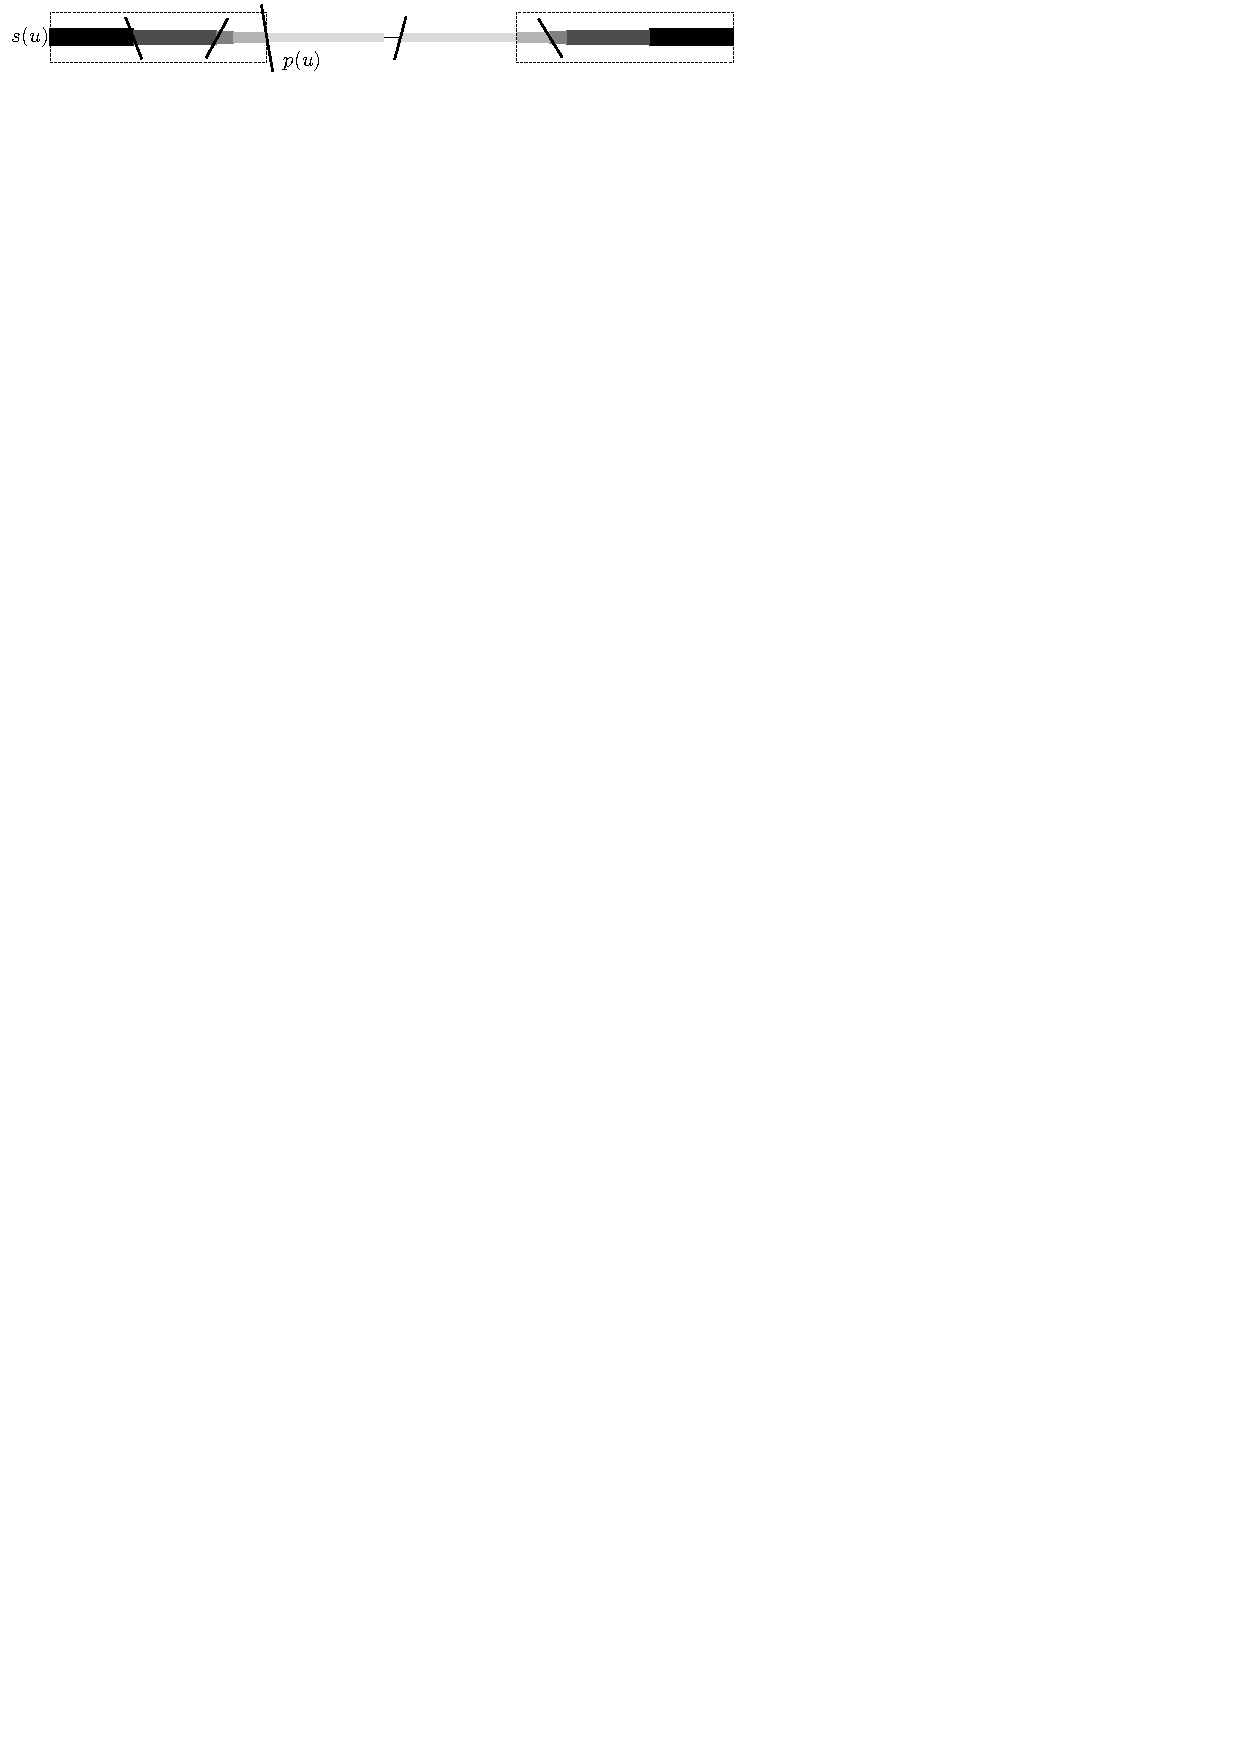
\includegraphics{figures/tree_illustration}
		\caption{A segment $s(u)$ with five intersecting segments and the different induced stub lengths. The boxed stub lengths are considered in $\solshort(u)$ and do not affect $p(u)$.} % The shaded areas are the stubs, $ p(u) $ is the parent of $ u $. The stubs in the boxed area contribute to $ \solshort(u) $.}
		\label{fig:tree}
	\end{figure}
	
	\subsection{Trees}
	\label{sec:tree}
	
	Here we assume that $ C =(V,E) $ is a rooted tree of maximum degree $ k $. 
	We give a bottom up dynamic programming algorithm for solving \maxsped on $ C $. 
	For each vertex $u \in V$ we compute and store the maximum ink values $T_i(u)$ for $i = 0, \dots, \delta$ with $\delta = \deg(u)$ for the subtree rooted at $u$ such that $s(u)$ is drawn as a pair of stubs of length $\ell_i(u)$.
	For $ u \in V $ let $ p(u) $ denote the parent of $ u $ in $ C $ and let $ c(u) $ denote the set of its children. 
	For $ u \in V $  %with parent $ p(u) \in V $ 
	let $ i_p $ be the index of the stub length $\ell_{i_p}(u)$ induced by the intersection point of $s(u)$ and $s(p(u))$.

	We define the following two values, which allow us to categorize the stub lengths into those not affecting the stubs of the parent and those that do affect the parent:
	\begin{align*}
		\solshort(u) = \max\{T_1(u),\dots,T_{i_p}(u)\}\\ % \qquad
		\sollong(u) = \max\{T_0(u),\dots,T_{\delta}(u)\}.
	\end{align*}
	Figure~\ref{fig:tree} highlights the stub lengths that are considered in $\solshort(u)$. We recursively define 
	\begin{align}
	\label{rec:tree}
	T_i(u) = \ell_i(u) + \sum_{v \in c(u)}
	\begin{cases}
	\solshort(v) & \text{if } s(u) \text{ with length } \ell_i(u) \text{ intersects } s(v) \\
	\sollong(v) & \text{otherwise}
	\end{cases}.
	\end{align}
	The correctness of Recurrence~(\ref{rec:tree}) follows by induction. 
	For a leaf $u$ in $C$ the set $c(u)$ is empty and the correctness of $T_i(u)$ is immediate.
	Further, $\solshort(u) = T_1(u)$ and $\sollong(u) = T_0(u)$ are set correctly for the parent $p(u)$.
	%Let $ C = (V,E) $ as above and $ u \in V $ a leaf of $ C $. Since $ c(u) $ is empty we simply get $ \solshort(u) = T_0(u) = \ell_1(u) $ and $ \sollong(u) = T_1(u) = \max\{\ell_0(u), \ell_1(u)\} $. 
	For an inner vertex $ u $ with degree $\delta$ we can assume by the induction hypothesis that the values $ \solshort(v) $ and $ \sollong(v) $ are computed correctly for all children $ v \in c(u) $. 
	Each value $ T_i(u) $ for $ 0 \leq i \leq \delta $ is then the stub length $ \ell_i(u) $ plus the sum of the maximum ink we can achieve among the children subject to the stubs of $u$ being drawn with length $\ell_i(u)$. 
	Setting $ \sollong(u) $ and $ \solshort(u) $ as above yields the two maximum ink values that are relevant for $ p(u) $.
	
	Recurrence~(\ref{rec:tree}) can be solved naively in $ O(mk^2) $ time, where $m = |V|$. 
	Using the order on the stub lengths  we can improve this to $ O(mk) $ time by computing all $ T_i(u) $ for one $ u \in V $ in $O(k)$ time.
	Let $u \in V$ be a vertex with degree $\deg(u) = \delta$. 
	The values $T_0(u) = \ell_0(u) + \sum_{v\in c(u)} \solshort(v)$ and $T_1(u) = \ell_1(u) + \sum_{v\in c(u)} \sollong(v)$ for the whole segment $s(u)$ and the shortest stubs can be computed in $O(k)$ time each.
	Now $T_{j+1}(u)$ can be computed from $T_j(u)$ in $O(1)$ time as follows.
	Let $v_j $ be the neighbor of $u$ that induces stub length $\ell_j(u)$ and assume $v_j \ne p(u)$.
	In $T_j(u)$ we could still count the value $\sollong(v_j)$, but in $T_{j+1}(u)$ the stub length of $u$ implies that $v_j$ can contribute only $\solshort(v_j)$. 
	Then $T_{j+1}(u) = T_j(u) - \sollong(v_j) + \solshort(v_j)$.
	If $v_j=p(u)$ the two values $T_j(u)$ and $T_{j+1}(u)$ are equal as the corresponding change in stub length has no effect on the children of $u$.
	Computing $\solshort(u)$ and $\sollong(u)$ clearly takes $O(k)$ time.
	
	So by solving Recurrence~(\ref{rec:tree}) in $O(mk)$ time we find an optimal solution to the \maxsped problem on $ G $ with drawing $ \Gamma $ using standard backtracking from $\max\{T_0(r), \dots, T_{\deg(r)}(r)\}$ for the root $r$ of $C$.	
	Since the intersection graph $C$ is a tree with $O(m)$ edges it can be computed in $O(m \log m)$ time and we obtain the following theorem.
	
	\begin{theorem}
		\label{thm:tree}
		Let $ G $ be a simple graph with $m$ edges and $ \Gamma $ a straight-line drawing of $ G $. If the intersection graph $ C = (V,E) $ of $ G $ is a tree with maximum degree $ k \in \mathbb{N} $, problem \maxsped can be solved in $ O(mk + m \log m) $ time and space.
	\end{theorem}

	\subsection{Cactus graphs}
	\label{sec:cactus}
	
	We now generalize our previous algorithm to cactus graphs. 
	Due to space constraints we provide only a sketch of the arguments and omit further details.
	Let the intersection graph $ C = (V,E) $ be a \emph{cactus graph}, i.e. a simple graph in which no edge $ e \in E $ is part of more than one cycle. 
	For a cactus graph $ C $ the \emph{block-cut tree} is an arbitrarily rooted tree $ \mathcal T = (\mathcal V, \mathcal E) $, where $ \mathcal V $ contains a node for every cycle and for every cut vertex in $ C $. 
	We call a node $ u \in \mathcal V $ a \emph{block node} if it represents an induced cycle on vertices $ V(u) \subseteq V $ and an \emph{articulation node} of the cut vertex $ a(u) = v \in V $ otherwise. 
	We have an edge $ uv \in \mathcal E $ between a block node $ u $ and an articulation node $ v $ whenever $ a(v) \in V(u) $ and an edge $ uv \in \mathcal E $ between two articulation nodes whenever $ a(u)a(v) \in E$. % is an edge in $ E $.
	We re-use the notation $p(u)$ and $c(u)$ to refer to the parent and to the children of a node $u \in \mathcal V$.
	
	We further define for each node $ u \in \mathcal V $ two indices $ i_p(u) \le i_q(u) $.  
	For an articulation node $u$, $i_p$ and $i_q$ are the indices corresponding to the stub lengths induced by the intersection points of $s(a(u))$ and its neighbors in $C$ among the vertex set of $p(u)$.
	For a block node $u$, $i_p$ and $i_q$ are the indices corresponding to the intersection points of the parent's segment $s(a(p(u)))$ with its neighbors in $V(u)$.
	Similar to Section~\ref{sec:tree} we now define three values for each articulation node $ u \in \mathcal V $ with degree $ \delta $:
	\begin{align*}
	\sollong(u) = \max\{T_0(u),\dots,T_\delta(u)\}\\
	\solmid(u) = \max\{T_1(u),\dots,T_{i_q}(u)\}\\
	\solshort(u) = \max\{T_1(u),\dots,T_{i_p}(u)\}.
	\end{align*}
	Further, we define the recurrence $T_i(u)$ for all articulation nodes $u \in \mathcal V$:
	\begin{align}
	\label{rec:cactus_articulation}
	T_i(u) = \ell_i(a(u)) + \sum_{v \in c(u)}
	\begin{cases}
	T_{i_p(v)}(v) & \text{if } 1 \le i < i_p(v)\\ %\ell_i(a(u)) \leq a \\
	T_{i_q(v)}(v) & \text{if } i_p(v) < i \leq i_q(v) \\
	T_{0}(v) & \text{otherwise}
	\end{cases}.
	\end{align}
	For a block node $ u \in \mathcal V $ we cut open the cycle it represents at vertex $a(p(u))$ (refer to Bruckdorfer et al.~\cite{bcgkmn-pped-17} for details) and consider the three relevant stub lengths of the parent's segment $s(a(p(u)))$ induced by $i_p(u)$ and $i_q(u)$ and the whole segment. 
	The resulting subgraph is a path on $V(u)$ with attached children that are articulation vertices in $\mathcal T$, so we can apply our algorithm of Section~\ref{sec:tree} with minor modifications.
	Once all values in the subgraph of block node $u$ are computed, we can derive the values $T_i(u)$ for the block node $u$.
	
	Correctness can be proved by modifying the inductive arguments of Section~\ref{sec:tree} accordingly. 
	Combining the linear running time for cycles of Bruckdorfer et al.~\cite{bcgkmn-pped-17} with the running time for trees of Theorem~\ref{thm:tree} we can argue that cactus graphs can in fact be handled in the same time and space bounds as trees.
	
	\begin{theorem}
		Let $ G $ be a simple graph with $m$ edges and $ \Gamma $ a straight-line drawing of $ G $. If the intersection graph $ C = (V,E) $ of $ G $ is a cactus with maximum degree $ k \in \mathbb{N} $, problem \maxsped can be solved in $ O(mk + m \log m) $ time and space.
	\end{theorem}
	
	\bibliography{paper}
\end{document}